% LaTex Template

\documentclass[12pt]{article}
%\usepackage{natbib}
\usepackage[letterpaper, margin=1.1in]{geometry}
\usepackage{graphicx}
\usepackage{wrapfig}
\usepackage{enumitem}
\setlist[enumerate]{itemsep=0mm}
\usepackage{multirow}
\usepackage{lscape}
\usepackage{caption}
\usepackage{subcaption}

\begin{document}
\noindent{Alexandra Pulwicki \\ \today}

\begin{center}
\Large \textbf{Appendix\\ Density}
\end{center}

tube vs depth - correction, new SP vs tube
elevation relation

\subsection*{Federal Sampler measurements and snow depth}

A plot of measured SWE and snow depth can be seen in Figure \ref{fig:tube_depth}. A positive linear relation exists (R$^2$ = 0.55). This positive relationship could be a result of physical processes, such as compaction and/or artifacts during data collection. The range of densities measured by the Federal sampler is large (225--410 kg m^{-3}) and the extreme values seem unlikely to exist at these study glaciers, which experience a continental snowpack with minimal mid-winter melt events. Furthermore, compaction effects would likely be small at these study glaciers because of the relatively shallow snowpack (deepest measurement was 285 cm). A plot of the depth-density relationship in snowpits can be seen in Figure \ref{fig:pit_depth}. No linear relationship exists between depth and snowpit-derived density (R$^2$ = 0.05). Together, these conditions lead to the likely conclusion that the Federal Sampler measurements are biased. 

To account for this likely artifact, the simplest form of linear detrending was applied. The linear fit was subtracted from each data point and the original data mean was added to each point. A plot of the detrended density data can be seen in Figure \ref{fig:tube_depthDETREND}. This detrended data will be used for all subsequent analysis. 

\begin{wrapfigure}{r}{0.75\textwidth} 
	\centering
	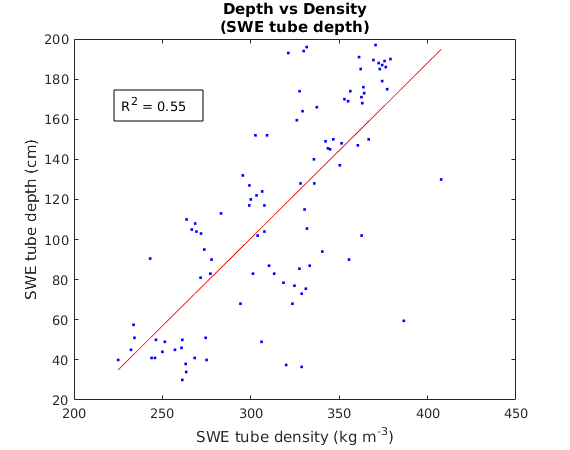
\includegraphics[width =0.75\textwidth]{DepthDensity_SWEtube.png}\\
	\caption{Relationship between measured density and snow depth for all Federal Sampler measurements.}
	\label{fig:tube_depth}
\end{wrapfigure}

\begin{wrapfigure}{R}{0.75\textwidth} 
	\centering
	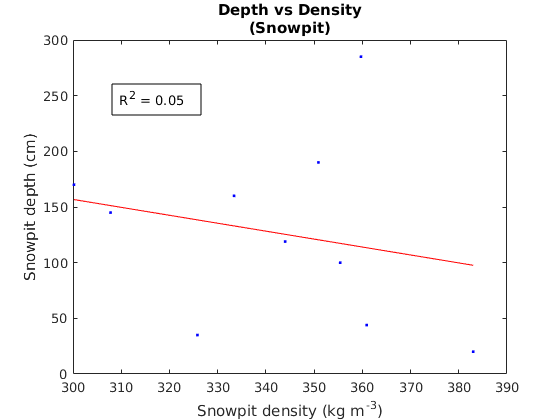
\includegraphics[width = 0.75\textwidth]{DepthDensity_SP.png}\\
	\caption{Relationship between measured density and snow depth for all snowpit locations.}
	\label{fig:pit_depth}
\end{wrapfigure}

\begin{wrapfigure}{r}{0.75\textwidth} 
	\centering
	\includegraphics[width =0.75\textwidth]{DepthDensity_tubeDENSITY.png}\\
	\caption{Detrended relationship between measured density and snow depth for all Federal Sampler measurements.}
	\label{fig:tube_depthDETREND}
\end{wrapfigure}


\subsection*{Basic statistics}

A summary of density data collected in snowpits and when using a Federal Sampler can be seen in Table \ref{tab:density_stats}. The standard deviation of each type of density measurement is also less than 10\% of the mean density. For snowpit derived densities, the mean density is indistinguishable between glaciers within one standard deviation. This was not observed in densities derived from Federal Sampler measurements --- Glacier 2 had the lowest mean density and Glacier 4 had the highest mean density. The mean of all Federal Sampler density values was likely skewed by the proportionally large number of measurements obtained on Glacier 13, and is thus indistinguishable from Glacier 13 mean density and different than both Glacier 4 and 2 mean density. 

\begin{table}[b!]
\centering
\caption{Mean, standard deviation (std), and number of measurements (n) of snow density measured on study glaciers in snowpits and using a Federal Sampler. }
\label{tab:density_stats}
\begin{tabular}{ccccccc}
\multirow{2}{*}{\textbf{Glacier}} & \multicolumn{3}{c}{\textbf{Snowpits}}     & \multicolumn{3}{c}{\textbf{Federal Sampler}} \\ 
                                  & Mean & Std & n & Mean  & Std  & n \\ \hline
\textbf{G04}                      & 348           & 13           & 3          & 360            & 10            & 7           \\
\textbf{G02}                      & 333           & 26           & 4          & 275            & 18            & 7           \\
\textbf{G13}                      & 349           & 26           & 3         & 321            & 9             & 17          \\
\textbf{All}                      & 342           & 26           & 10         & 321            & 9             & 31         
\end{tabular}
\end{table}

\subsection*{Density uncertainties}

\subsubsection*{Snowpit density}

Uncertainty in estimating density from snowpits is likely dominated by measurement errors and incorrect assumptions of density of layers that could not be sampled (i.e. ice lenses and 'hard' layers). To determine a possible range of density values from snowpit measurements, the original data was used and three parameters were varied. Ice layer density was varied between 700 and 900 kg m$^{-3}$, ice layer thickness was varied by $\pm$1 cm, and the density of layers identified as being too hard to sample (but not ice) between 600 and 700 kg m$^{-3}$. The resulting minimum and maximum possible densities for each snowpit can be seen in Table \ref{tab:density_pitrange}. The range of density values is always less than 10\% of the reference density (except for `G02\_LSP'). Density values for shallow pits that contained ice lenses were particularly sensitive to changes in density and ice lens thickness. 

\begin{table}[]
\centering
\caption{Range of snowpit density estimates. Minimum and maximum density values derived from varying ice layer density between 700 and 900 kg m$^{-3}$, ice layer thickness by $\pm$1 cm, and the density of layers identified as being too hard to sample (but not ice) between 600 and 700 kg m$^{-3}$. Reference values are those used in future analysis and were determined using an ice density of 900 kg m$^{-3}$, the recorded ice thickness, and a `hard' layer density of 600 kg m$^{-3}$.}
\label{tab:density_pitrange}
\begin{tabular}{lccccc}
\multicolumn{1}{c}{\multirow{2}{*}{\textbf{Snowpit}}} & \multicolumn{3}{c}{\textbf{Density (kg m$^{-3}$)}} & \multirow{2}{*}{\textbf{\begin{tabular}[c]{@{}c@{}}Range as \% \\ of mean (\%)\end{tabular}}} & \multirow{2}{*}{\textbf{\begin{tabular}[c]{@{}c@{}}Snowpit \\ depth (cm)\end{tabular}}} \\
\multicolumn{1}{c}{} & Mean & Minimum & Maximum &  &  \\ \hline
G02\_LSP & 361 & 329 & 377 & 13 & 44 \\
G02\_Z4A\_SWE & 326 & 308 & 345 & 11 & 35 \\
G02\_USP & 344 & 327 & 362 & 10 & 119 \\
G02\_ASP & 300 & 299 & 303 & 1 & 170 \\
G04\_LSP & 351 & 343 & 359 & 5 & 190 \\
G04\_USP & 333 & 317 & 350 & 10 & 160 \\
G04\_ASP & 360 & 357 & 362 & 1 & 285 \\
G13\_LSP & 383 & 383 & 383 & 0 & 20 \\
G13\_USP & 355 & 346 & 367 & 6 & 100 \\
G13\_ASP & 308 & 306 & 308 & 1 & 145
\end{tabular}
\end{table}

\subsubsection*{Federal Sampler densities}

Density values estimated from Federal Sampler measurements are shown in Table \ref{tab:density_TubeRange}. Mean density is has a larger spread of values when compared to snowpit densities across the study area. The \% range is also larger than snowpit densities for many of the measurement locations. 

\begin{table}[]
\centering
\caption{Range of densities estimated from Federal Sampler measurements. The number (n) of good quality measurements, as well as the minimum, maximum, and mean density are shown. The density range given as a percent of the mean density is also shown.}
\label{tab:density_TubeRange}
\begin{tabular}{lccccc}
\multicolumn{1}{c}{\multirow{2}{*}{\textbf{Glacier}}} & \multirow{2}{*}{\textbf{n}} & \multicolumn{3}{c}{\textbf{Density (kg m$^{-3}$)\}}} & \multirow{2}{*}{\textbf{\begin{tabular}[c]{@{}c@{}}Range as \\ \% of mean (\%)\end{tabular}}} \\
\multicolumn{1}{c}{} &  & Mean & Minimum & Maximum &  \\ \hline
G04\_Z3A\_SWE & 3 & 370 & 361 & 379 & 5 \\
G04\_USP & 6 & 352 & 328 & 364 & 10 \\
G04\_Z2A\_SWE & 3 & 368 & 353 & 377 & 7 \\
G04\_LSP & 7 & 372 & 362 & 376 & 4 \\
G04\_Z5B\_SWE & 2 & 359 & 356 & 363 & 2 \\
G04\_Z5A\_SWE & 3 & 328 & 321 & 332 & 3 \\
G04\_Z5C\_SWE & 2 & 332 & 328 & 336 & 2 \\
G02\_Z5C\_SWE & 2 & 273 & 264 & 283 & 7 \\
G02\_USP & 7 & 283 & 267 & 308 & 14 \\
G02\_Z7A\_SWE & 3 & 342 & 326 & 369 & 13 \\
G02\_Z7B\_SWE & 2 & 306 & 303 & 309 & 2 \\
G02\_Z7C\_SWE & 3 & 300 & 295 & 306 & 4 \\
G02\_Z3B\_SWE & 3 & 243 & 232 & 251 & 8 \\
G02\_LSP & 7 & 251 & 234 & 263 & 12 \\
G13\_ASP & 8 & 349 & 342 & 361 & 5 \\
G13\_651 & 3 & 352 & 344 & 367 & 7 \\
G13\_652 & 2 & 343 & 330 & 356 & 8 \\
G13\_654 & 3 & 335 & 294 & 387 & 28 \\
G13\_655 & 1 & 340 & 340 & 340 & 0 \\
G13\_656 & 3 & 336 & 313 & 363 & 15 \\
G13\_657 & 3 & 304 & 263 & 329 & 22 \\
G13\_658 & 2 & 319 & 303 & 336 & 10 \\
G13\_659 & 3 & 314 & 304 & 332 & 9 \\
G13\_Z7C\_SWE & 2 & 274 & 272 & 277 & 2 \\
G13\_USP & 6 & 317 & 301 & 331 & 9 \\
G13\_Z4C\_SWE & 1 & 408 & 408 & 408 & 0 \\
G13\_744 & 3 & 240 & 225 & 250 & 10 \\
G13\_Z3B\_SWE & 3 & 268 & 261 & 275 & 5 \\
G13\_Z4B\_SWE & 2 & 290 & 275 & 306 & 11 \\
G13\_Z5A\_SWE & 3 & 265 & 243 & 278 & 13 \\
G13\_Z5B\_SWE & 2 & 322 & 318 & 325 & 2
\end{tabular}
\end{table}



\subsection*{Comparing density from snowpit and Federal Sampler measurements}

To compare snowpit-derived densities and Federal Sampler-derived densities, eight Federal Sampler measurements were taken around two snowpit locations on each study glacier. The results are seen in Figure \ref{fig:density_pitVStube}. The overall range of Federal Sampler-derived densities is considerably larger than that of the snowpit-derived density values. A linear regression of the data gives a weak inverse relationship (R$^2$ = 0.24).

\begin{wrapfigure}{r}{\textwidth} 
	\centering
	\fbox{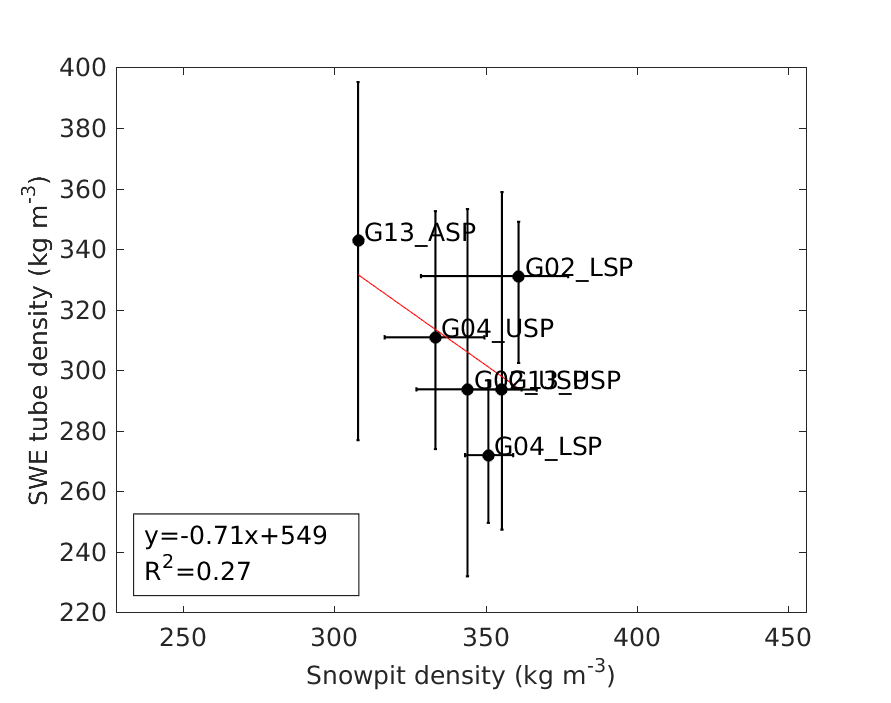
\includegraphics[width = \textwidth]{SnowpitVsSWEtube_all.png}}\\
	\caption{Comparison of density estimated using wedge cutters in a snow pit and Federal Sampler measurements for three study glacier (G04, G02, G13). Error bars are minimum and maximum values for each estimate as seen in Table \ref{tab:density_pitrange} and \ref{tab:density_TubeRange}.}
	\label{fig:density_pitVStube}
\end{wrapfigure}




\begin{enumerate}
\item 
\end{enumerate}










\end{document}